
\begin{frame}
  \frametitle{Évolution des Processeurs Graphiques}
  \begin{center}
    \begin{tikzpicture}[yscale=-1]
      % \draw[help lines] (0,0) grid (15,6);
      % > latex arroxw
      \draw[line width=10pt,-latex] (1.5,1) .. controls +(1,4) and +(-5,-0) .. +(10,4);
      \node at (1.5,1) {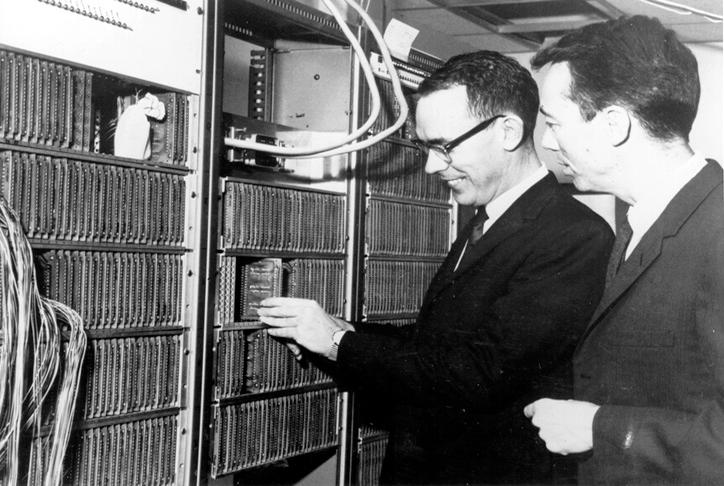
\includegraphics[scale=.1]{images/evans-sutherland.jpg}};
      \node [anchor=south,align=center] at (1.5,0) {Evan \& Sutherland \\ {\small 1970}};
      \node at (3,3.25) {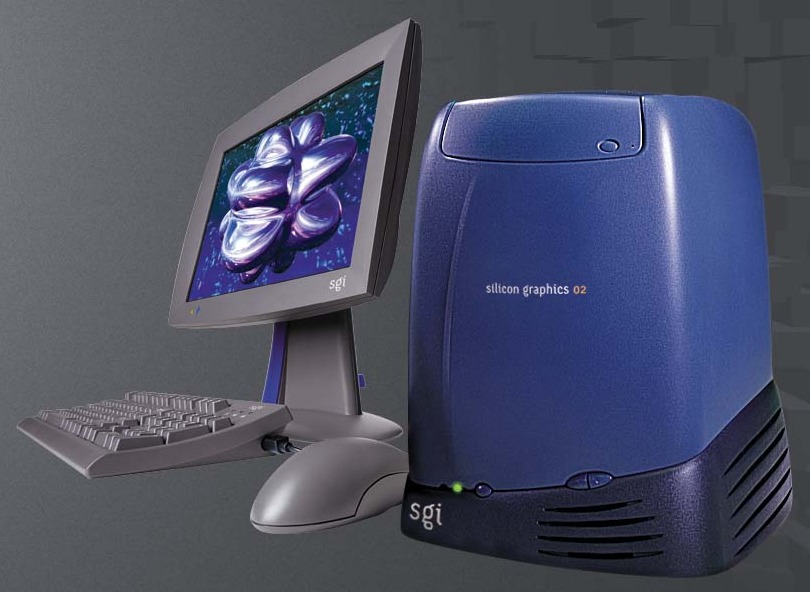
\includegraphics[scale=.1]{images/sgi-o2-workstation.jpg}};
      \node [anchor=north,align=center] at (2.5,4.25) {SGI Workstation \\ {\small 1990-2004}};
      \node at (6,4.75) {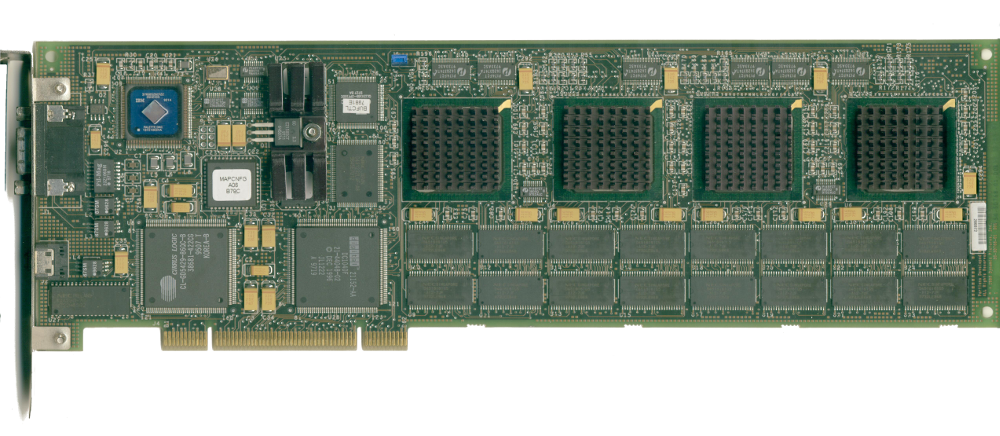
\includegraphics[scale=.5]{images/oxygen.png}};
      \node [anchor=north] at (6,5.25) {Accélérateur Graphique};
      \node at (9,5) {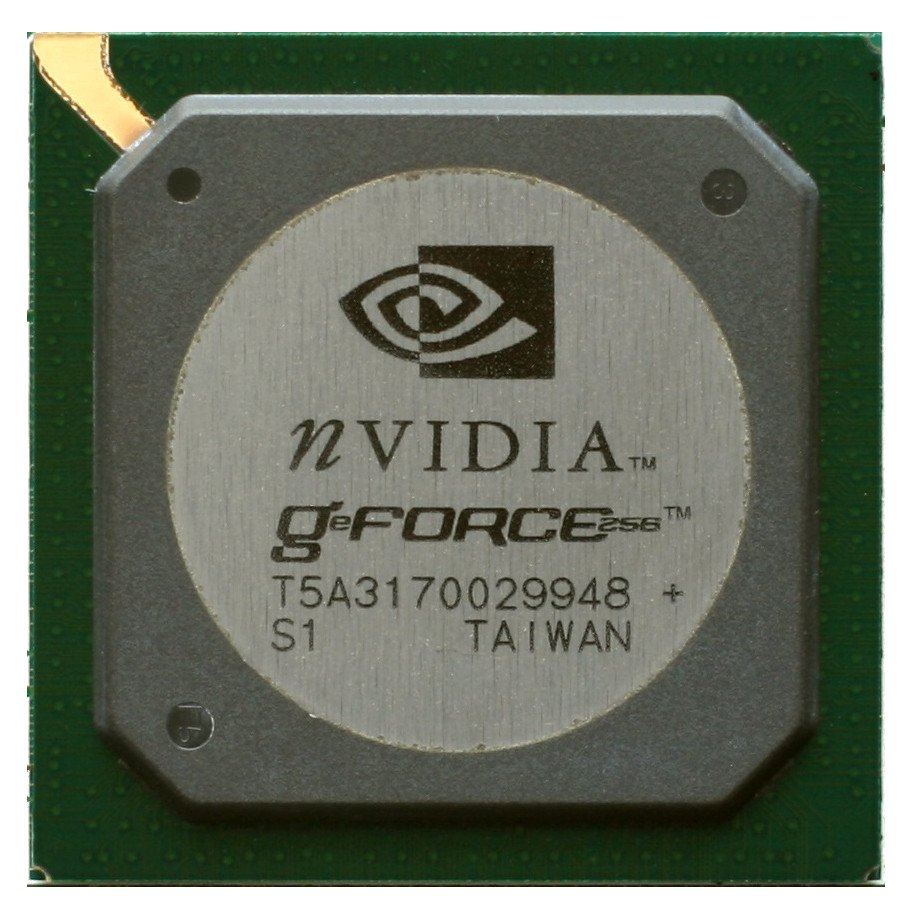
\includegraphics[scale=.03]{images/nvidia-gforce.png}};
      \node [anchor=south,align=center] at (9,4.5) {Nvidia GeForce 256 \\ $1^\text{er}$ GPU \\ {\small 2000}};
      \node [anchor=west,align=left] at (11.5,5) {\textbf{General Purpose} \\ \textbf{GPU} \\ {\small 2006}};
      \draw (14.5,0) -- +(.01,0); % hack
    \end{tikzpicture}
  \end{center}
  \begin{textblock}{12}(5,2)
    \textbf{Convergence}
    \begin{itemize}
    \item du hardware professionnel et grand-publique
    \item des processeurs graphiques et de calculs
    \item des plateformes~: de l'embarqué au super-calculateur 
    \end{itemize}
  \end{textblock}
  %%%%%%%%%%
  \note{
    \begin{enumerate}
    \item des pionniers aux machines spécifiques
    \item aux stations de travail professionnels
    \item à présent plus de distinction
    \item I. Sutherland (left) and D. Evans (right) with Line Drawing System-1. December 1969.
    \end{enumerate}
  }
\end{frame}

\begin{frame}
  % \frametitle{Présentation des GPUs~: processeurs de flux}
  \frametitle{Qeulques mots sur les GPUs}
  % dessin flux de données traversant la page
  \begin{center}
    % \begin{tabular}{>{\centering\arraybackslash}m{.4\textwidth} >{\centering\arraybackslash}m{.4\textwidth}}
    % tikz bbox
    \begin{tabular}{m{8cm}m{35mm}}
      \centerline{Intel Haswell Die} & \centerline{Nvidia Kepler Die} \\
      \centerline{\begin{tikzpicture}[mystyle/.style={-latex, line width=1pt}]
        \node (0,0) {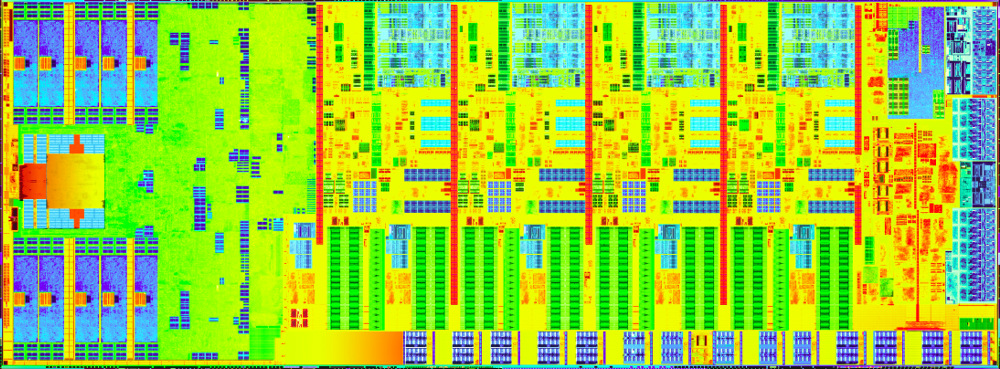
\includegraphics[height=.3\textheight]{images/intel-haswell-die.jpg}};
        \node (o1) at (-3.75,1.5) {\tiny GPU core};
        \draw[mystyle] (o1) -- ++(.5,-.5);
        \node (o2) at (-1.75,1.5) {\tiny CPU core};
        \draw[mystyle] (o2) -- ++(1,-1);
        \node (o3) at (-.7,-1.5) {\tiny L3 Cache};
        \draw[mystyle] (o3) -- ++(1,.75);
      \end{tikzpicture}} &
      \centerline{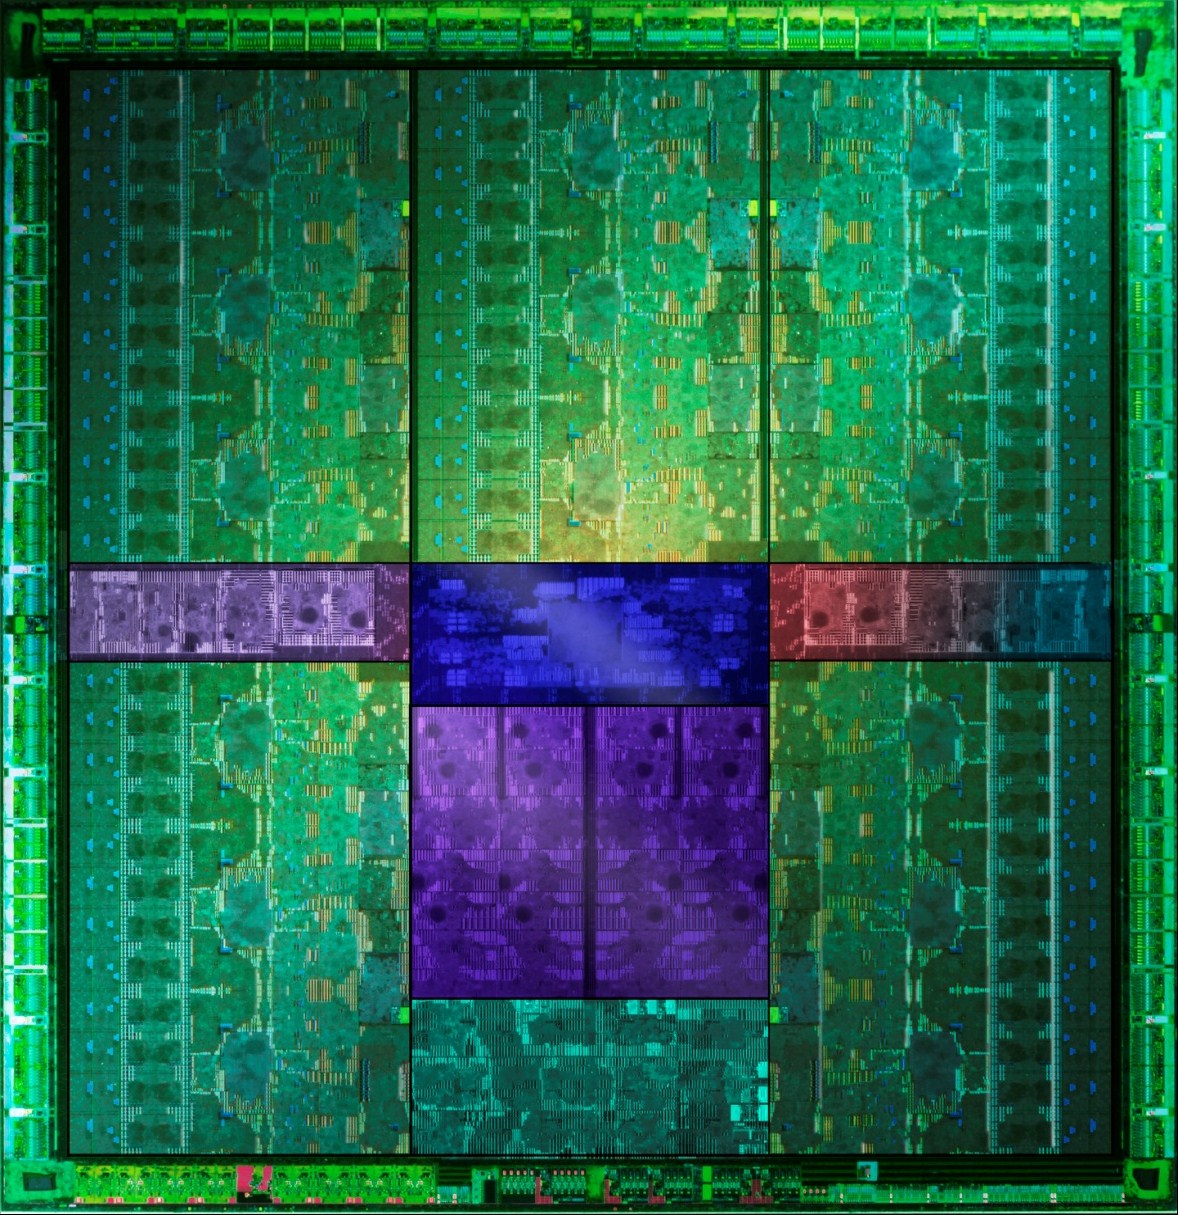
\includegraphics[height=.3\textheight]{images/nvidia-kepler-die.jpg}}
    \end{tabular} \\
    \begin{minipage}{.7\linewidth}
      Architecture de calcul ($\times$, $+$) hautement parallèle \\
      des interpolateurs de lignes et de triangles \\
      couplée à une mémoire rapide (GDDR5)
    \end{minipage}
  \end{center}
  %%%%%%%%%%
  \note{
    \begin{enumerate}
    \item c'est quoi un GPU
    \item CPU~: usage générique
    \item SIMD AVX2 256-bit 8x float 32-bit
    \item flux de données
    \item pas la même architecture, cf.\ silicium
    \end{enumerate}
  }
\end{frame}

\begin{frame}
  \frametitle{Usage des GPUs}
  % keywords picture
  % pgf mindmap cf. p75
  \begin{columns}
    \begin{column}{.2\textwidth}
      \begin{center}
        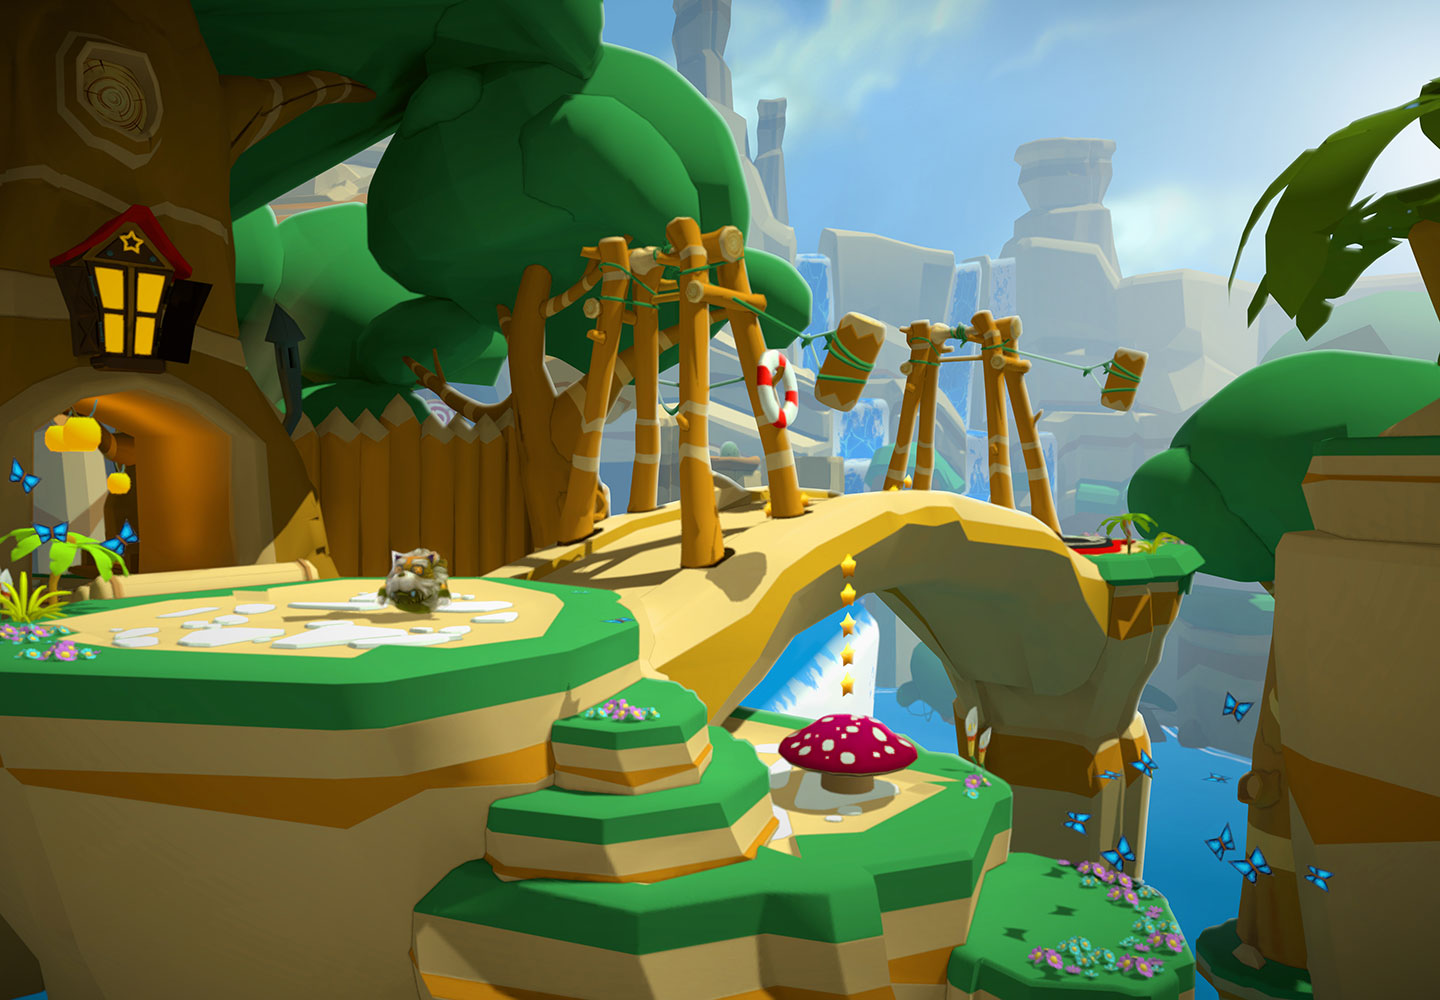
\includegraphics[width=1.\textwidth]{images/game.jpg} \\[5mm]
        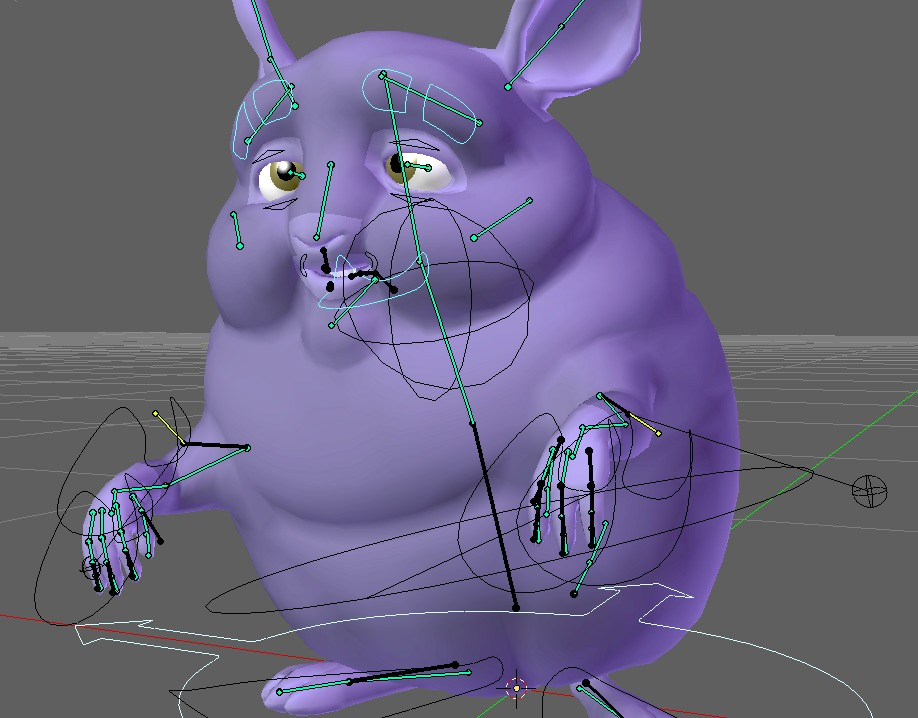
\includegraphics[width=1.\textwidth]{images/blender.jpg}
      \end{center}
    \end{column}
    \begin{column}{.2\textwidth}
      \begin{center}
        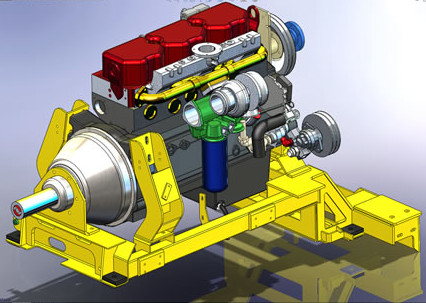
\includegraphics[width=1.\textwidth]{images/solidworks.jpg} \\[5mm]
        
\includegraphics[width=.8\textwidth]{images/tiger.jpg}
      \end{center}
    \end{column}
    \begin{column}{.1\textwidth}
      \begin{center}
        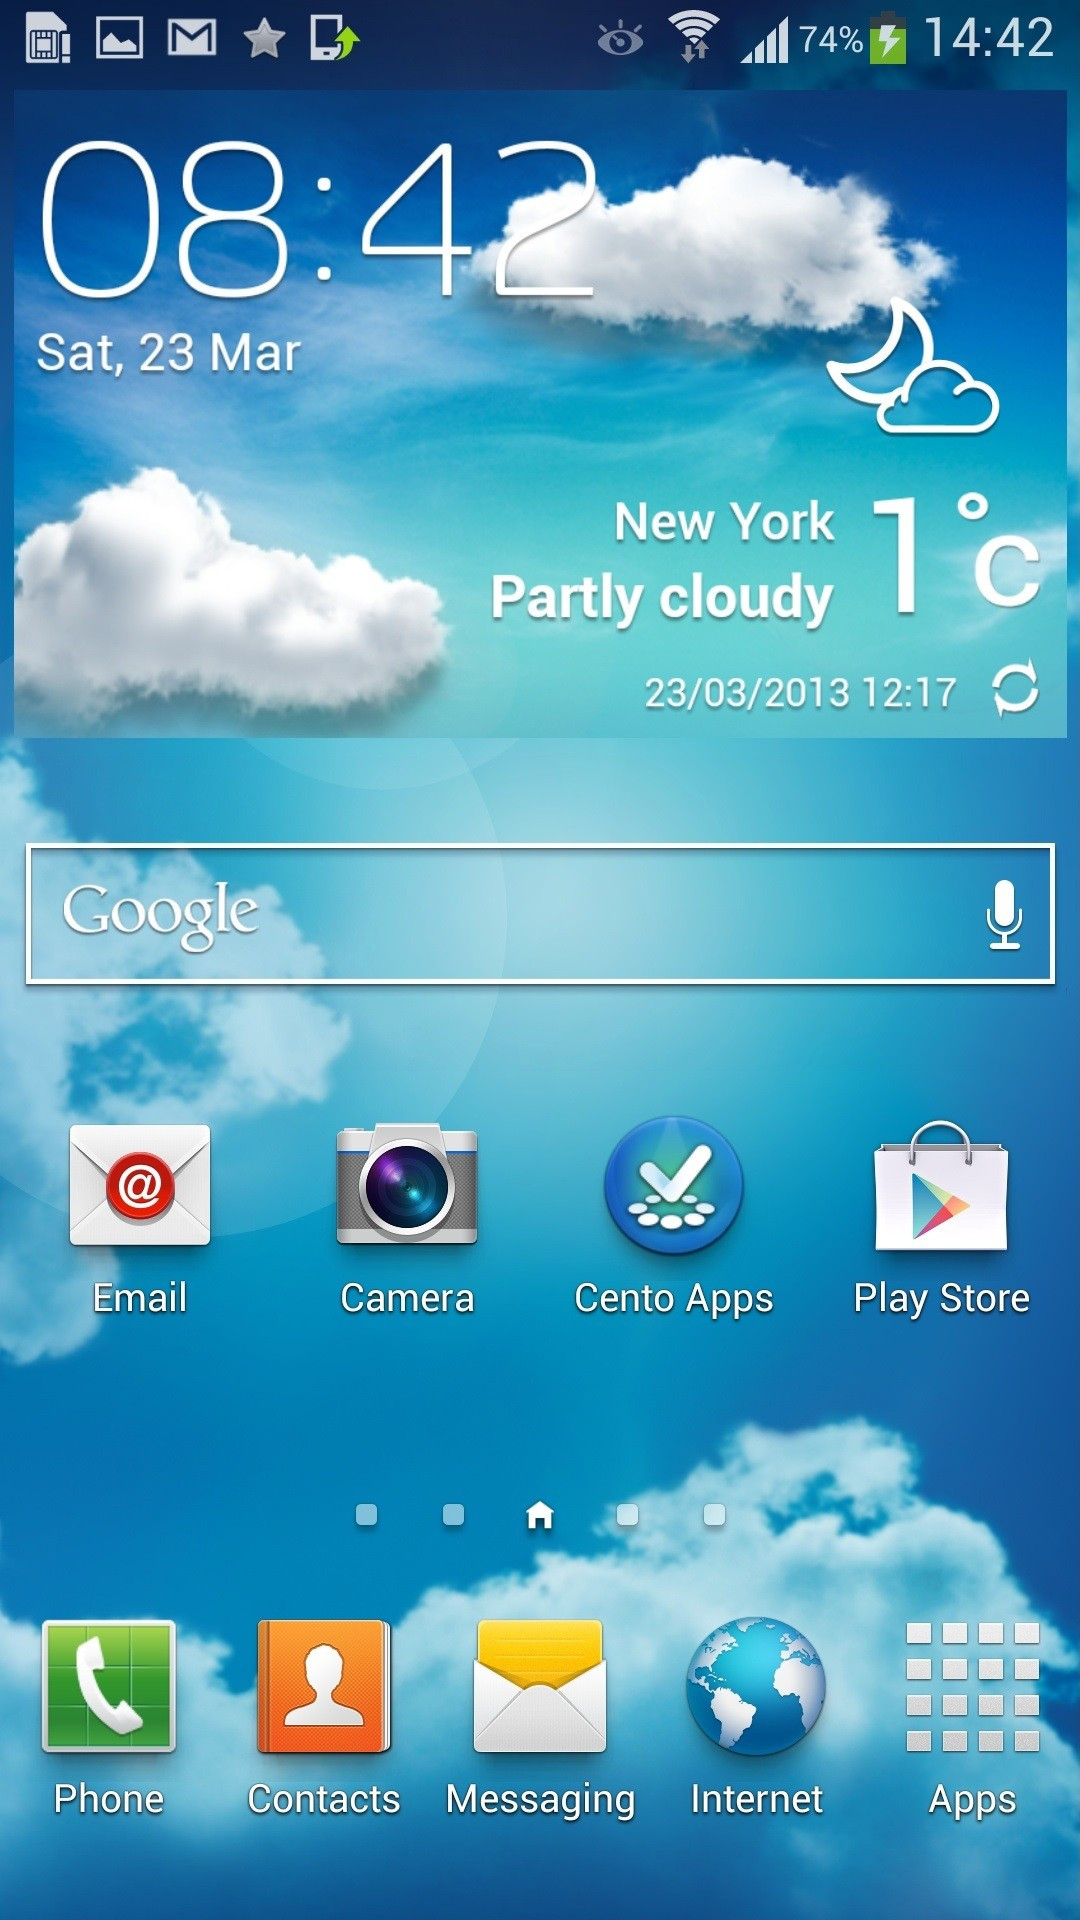
\includegraphics[height=2.5cm]{images/touchwiz.jpg}
      \end{center}
    \end{column}
    \begin{column}{.4\textwidth}
      \begin{itemize}
      \item Moteur de jeu % Game Engine
      \item Modeleur \textbf{3D}
      \item CAO
      \item \textbf{Visualisation} scientifique
      \item \textbf{Interface graphique} \\
        e.g.\ Qt QML, KDE Plasma
      \item \textbf{2D} avec accélération matériel
      \item \textbf{Calcul}~: CUDA, OpenCL
      \end{itemize}
    \end{column}
  \end{columns}
  %%%%%%%%%%
  \note{
    \begin{enumerate}
      \item Qu'est ce que l'on peut faire avec un GPU?
      \item OpenVG, SVG, Display Postscript
    \end{enumerate}
  }
\end{frame}

\begin{frame}
  \frametitle{Présentation de l'API \href{http://www.opengl.org}{OpenGL}}
  \begin{columns}
    \begin{column}{.2\textwidth}
      \begin{center}
        
\includegraphics[width=1.\textwidth]{images/khronos-logos/OpenGL/OpenGL_500.jpg} \\
        
\includegraphics[width=1.\textwidth]{images/khronos-logos/OpenGL_ES/OpenGL-ES_500.jpg} \\
        
\includegraphics[width=1.\textwidth]{images/khronos-logos/WebGL/WebGL_500.jpg} \\
        
\includegraphics[width=1.\textwidth]{images/khronos-logos/Khronos_Group/Khronos_Group_500.jpg}
      \end{center}
    \end{column}
    \begin{column}{.8\textwidth}
      \begin{itemize}
      \item Un standard \textbf{ouvert} gouverné par le groupe \href{http://www.khronos.org}{Khronos}
      \item La seule API \textbf{cross-platforme} et \textbf{cross-vendor} % cross / multi
      \item L'API de facto de GNU/Linux et d'Android
      \item Une API orientée desktop (OpenGL) et embarqué (OpenGL ES)
      \item et aussi orientée web (WebGL)
      \item \alert{Mais pas un idéale} cf.\ \href{https://www.khronos.org/assets/uploads/developers/library/2014-siggraph-bof/OpenGL-Ecosystem-BOF_Aug14.pdf}{Siggraph 2014 Khronos talk}
        % \url{https://www.khronos.org/developers/library/2014-siggraph-bof}
      \end{itemize}
    \end{column}
  \end{columns}
  %%%%%%%%%%
  \note{
    \begin{enumerate}
    \item C'est quoi OpenGL?
    \item Next generation OpenGL initiative
    \end{enumerate}
  }
\end{frame}

\begin{frame}
  \frametitle{Évolution de l'API OpenGL~: 20 ans d'existence}
  \begin{columns}
    \begin{column}{.7\textwidth}
      \begin{center}
        \includegraphics[width=1.\textwidth]{figures/opengl-release-date.pdf} % ,transparent
      \end{center}
    \end{column}
    \begin{column}{.3\textwidth}
      \textbf{Déphasage} entre \\
      \begin{itemize}
      \item OpenGL
      \item Hardware
      \item machine de l'utilisateur
      \item \href{http://www.mesa3d.org}{Mesa}
      \item programmeur
      \end{itemize}
      \alert{Quelle API choisir?}
    \end{column}
  \end{columns}
    \begin{center}
      \alert{Toujours actif, mais concurrencé~: DirectX 12, AMD Mantle, Apple Metal \ldots}
    \end{center}
  %%%%%%%%%%
  \note{
    \begin{enumerate}
    \item 20 ans d'histoire
    \item dynamique des releases
    \item concept d'extension pour expérimenter
    \end{enumerate}
  }
\end{frame}

\begin{frame}
  \frametitle{Implémentations}
  \begin{columns}
    \begin{column}{.5\textwidth}
      \begin{center}
        \href{http://mesamatrix.net}{Status de Mesa} pour l'Intel HD Graphics {\tiny (*)} \\[.5em]
        \includegraphics[width=1.\textwidth]{figures/mesa-status.pdf} \\ % ,transparent
      \end{center}
      {\tiny (*) core i3/5/7}
    \end{column}
    \begin{column}{.5\textwidth}
      \begin{itemize}
      \item {\small Extensions~: \\
        ensemble de nouvelles fonctions \\
        avant leurs intégrations dans l'API core}
      \item \href{http://www.mesa3d.org}{Mesa}~: OpenGL sous Linux \\
        à 2 doigts d'OpenGL V4.0
      \item Nvidia implémente 99,9\,\% de l'API % OpenGL driver
      \end{itemize}
    \end{column}
  \end{columns}
  %%%%%%%%%%
  \note{
    \begin{enumerate}
    \item Quelle API cibler pour développer une application?
    \end{enumerate}
  }
\end{frame}

\begin{frame}[fragile]
  \frametitle{Programmable Pipeline}
  \begin{center}
    OpenGL Moderne $=$ Calcul Générique $+$ Graphic Stuffs \\[1em]
    flux de vertex $\longrightarrow$ ligne / triangle $\longrightarrow$ pixels
  \end{center}
  \begin{columns}
    \begin{column}{.5\textwidth}
      \begin{itemize}
      \item programme~: shader
      \item constantes~: \boxR{uniform} \\
        e.g.\ float, matrice \\
        interpolateur d'images 1D/2D/3D
      \item données~: \boxG{in} \\
        sous formes de flux (array) \\
        vecteur 1D/2D/3D
      \item résultat~: \boxB{out}
      \end{itemize}
    \end{column}
    \begin{column}{.4\textwidth}
      \begin{center}
        Shader GLSL
        \rule{\textwidth}{1pt}
        % \framebox
{\scriptsize%
\begin{Verbatim}[commandchars=\\\{\}]
\boxR{uniform} mat4 model_view_matrix;
\boxR{uniform} mat3 normal_matrix;
\boxR{uniform} usampler2D texture0;

\boxG{in} vec3 position;
\boxG{in} vec3 normal;

\boxB{out} vec4 fragment_colour;

void main() \{
  ...
  fragment_colour = ...;
\}
\end{Verbatim}
}
      \end{center}
    \end{column}
  \end{columns}
  \begin{tikzpicture}[remember picture, overlay, mystyle/.style={-latex, line width=1pt}] % run % twice
    \node (o1) at ($(current page.south west) + (7,4.5)$) {Numpy Array};
    \draw[mystyle] (o1) -- ($(current page.south west) + (9,4.5)$);
    \draw[mystyle] (o1) -- ($(current page.south west) + (9,3)$);
  \end{tikzpicture}
  %%%%%%%%%%
  \note{
    \begin{enumerate}
    \item expliquer le passage fixed pipeline $\longrightarrow$ programmable pipeline
    \item concepts
    \item comment on utilise OpenGL depuis Python
    \end{enumerate}
  }
\end{frame}

\begin{frame}
  \frametitle{Outils pour interfacer du code C avec Python}
  \begin{center}
    % \begin{tabular}{|c|c|c|}
    \begin{tabular}{lccc}
      & Avantages & Inconvénients & Pypy \\[.5em]
      %
      \colorB{\href{https://docs.python.org/3.4/c-api}{API C Python}} &
      \begin{minipage}[t]{.2\linewidth}
        \tiny
        \begin{itemize}
        \item au coeur de CPython
        \end{itemize}
      \end{minipage} &
      \begin{minipage}[t]{.45\linewidth}
        \tiny
        \begin{itemize}
        \item implémentation manuelle
        \item requiert un compilateur
        \end{itemize}
      \end{minipage} &
      \textcolor{orange}{Non} \\[1em] % ???
      %\hline
      %
      \begin{minipage}[t]{2cm}
        \colorB{\href{http://www.swig.org}{SWIG}} \\
        \tiny{$=$ API C automatisé}
      \end{minipage} &
      \begin{minipage}[t]{.2\linewidth}
        \tiny
        \begin{itemize}
        \item \textbf{header parser}
        \item \textbf{supporte \Cpp}
        \item multi-langages
        \end{itemize}
      \end{minipage} &
      \begin{minipage}[t]{.45\linewidth}
        \tiny
        \begin{itemize}
        \item le mécanisme de macros (typemap) engendre du code bloat
        \item pas optimisé pour un langage
        \end{itemize}
      \end{minipage} &
      \textcolor{orange}{Non} \\[1em] % ???
      %\hline
      %
      \colorG{\href{https://docs.python.org/3.4/library/ctypes.html}{Ctypes}} &
      \begin{minipage}[t]{.2\linewidth}
        \tiny
        \begin{itemize}
        \item \textbf{inclus dans CPython}
        \end{itemize}
      \end{minipage} &
      \begin{minipage}[t]{.45\linewidth}
        \tiny
        \begin{itemize}
          \item pas d'header parser
          \item pas d'API level
        \end{itemize}
      \end{minipage} &
      \textcolor{red}{Non} \\[1em]
      %\hline
      %
      \colorG{\href{https://cffi.readthedocs.org/en/release-0.8}{Cffi}} &
      \begin{minipage}[t]{.2\linewidth}
        \tiny
        \begin{itemize}
        \item \textbf{header parser}
        \item \textbf{ABI et API level}
        \end{itemize}
      \end{minipage} &
      \begin{minipage}[t]{.45\linewidth}
        \tiny
        \begin{itemize}
        \item ???
        \end{itemize}
      \end{minipage} &
    \textcolor{green}{Oui}
    \end{tabular} \\[2em]
    \alert{Cffi est la solution idéale pour interfacer du C} \\[.5em]
    \alert{SWIG est une solution pour interfacer du \Cpp} \\[.5em]
    % \alert{L'idéale pour \Cpp{} est la réflexion}
    \alert{mais l'idéale serait la réflexion}
  \end{center}
  \begin{textblock}{5}(14,8)
    \tiny mais aussi\\
    \href{http://www.riverbankcomputing.com/software/sip/intro}{sip}
    \href{http://www.cosc.canterbury.ac.nz/greg.ewing/python/Pyrex/}{Pyrex}
  \end{textblock}
  \begin{textblock}{5}(1,8)
  \colorG{$\star$ \href{https://sourceware.org/libffi}{libffi}}
  \end{textblock}
  %%%%%%%%%% 
  \note{
    \begin{enumerate}
    \item Comment on lie une bibliothèque à Python
    \end{enumerate}
  }
\end{frame}

\begin{frame}[fragile]
  \frametitle{\href{http://pyopengl.sourceforge.net}{PyOpenGL}~: la réference actuelle}
  3 générations~:
  \begin{description}
    \item[V1.x] C extension basé sur l'API C Python {\tiny (David Ascher et. al)}
    \item[V2.x] généré par SWIG {\tiny (Tarn Weisner Burton)}
    \item[V3.x] basé sur ctypes et un header parser % de fichier d'en-tête
      {\tiny (\href{http://www.vrplumber.com}{Mike C. Fletcher})} \\
      \textbf{compatibilité ascendante avec la V2.x}
    \end{description}
    \vspace{1em}
    et des alternatives plus spécifique~:
    \begin{description}
    \item[\href{http://www.pyglet.org}{Pyglet}] a cross-platform windowing and multimedia library
    \item[\href{http://vispy.org}{Vispy}] a high-performance interactive 2D/3D data visualization library
    \end{description}
  %%%%%%%%%%
  \note{
    \begin{enumerate}
    \item Présentation de l'existant
    \end{enumerate}
  }
\end{frame}

\begin{frame}[fragile]
  \frametitle{PyOpenGL~: ce qui pêche}
  Exemples de difficultés rencontrées au cours du temps~:
    \begin{itemize}
    \item absence de constante~:%
      {\tiny\begin{verbatim}GL.GL_RG_INTEGER = OpenGL.constant.Constant('GL_RG_INTEGER', 0x8228)}\end{verbatim}}
    \item \code{glGetObjectParameteriv} est ici~:%
      {\tiny\begin{verbatim}import OpenGL.GL.ARB.shader_objects as GL_SO\end{verbatim}}
    \item \code{glGetActiveUniformBlockName} n'a pas de Pythonic wrapper~:
{\tiny%
\begin{verbatim}
name = ctypes.create_string_buffer(max_name_length)
name_length = OpenGL.arrays.GLsizeiArray.zeros((1,))
GL.glGetActiveUniformBlockName(program, index, max_name_length, name_length, name)
return name.value[:int(name_length[0])]
\end{verbatim}}
    \end{itemize}
    \vspace{1em}
    En résumé~:
    \begin{itemize}
    \item \textbf{une longue histoire}
    \item un code source touffu~: 2000 fichiers \small({\emph{en comptant les extensions})}
      % {\tiny et PyOpenGL-accelerate}
    \item Python et OpenGL ont évolué
    \item pas d'API de haut niveau pour l'OpenGL moderne % l'API 
    \end{itemize}
  %%%%%%%%%%
  \note{
    \begin{enumerate}
    \item Pourquoi réimplémenter PyOpenGL
    \end{enumerate}
  }
\end{frame}

%%% Local Variables: 
%%% mode: latex
%%% TeX-master: "master"
%%% End: 
